\documentclass[tikz,border=4pt]{standalone}
% Paleta y fuentes compartidas por el libro y las figuras (única fuente de verdad).
\RequirePackage{xcolor}
\definecolor{oxido}{HTML}{B7410E}
\definecolor{cobre}{HTML}{D27D2D}
\definecolor{carbon}{HTML}{2B2B2B}
\definecolor{azul}{HTML}{1F5F8B}
\definecolor{arena}{HTML}{F4EDE4}

\usepackage{fontspec}
\setsansfont{FiraSans}[Extension=.otf,UprightFont=*-Regular,BoldFont=*-Bold,ItalicFont=*-Italic,BoldItalicFont=*-BoldItalic]
\setmonofont{FiraMono}[Extension=.otf,UprightFont=*-Regular,BoldFont=*-Medium]
\usetikzlibrary{positioning,arrows.meta,calc,fit}
\begin{document}
\sffamily\small
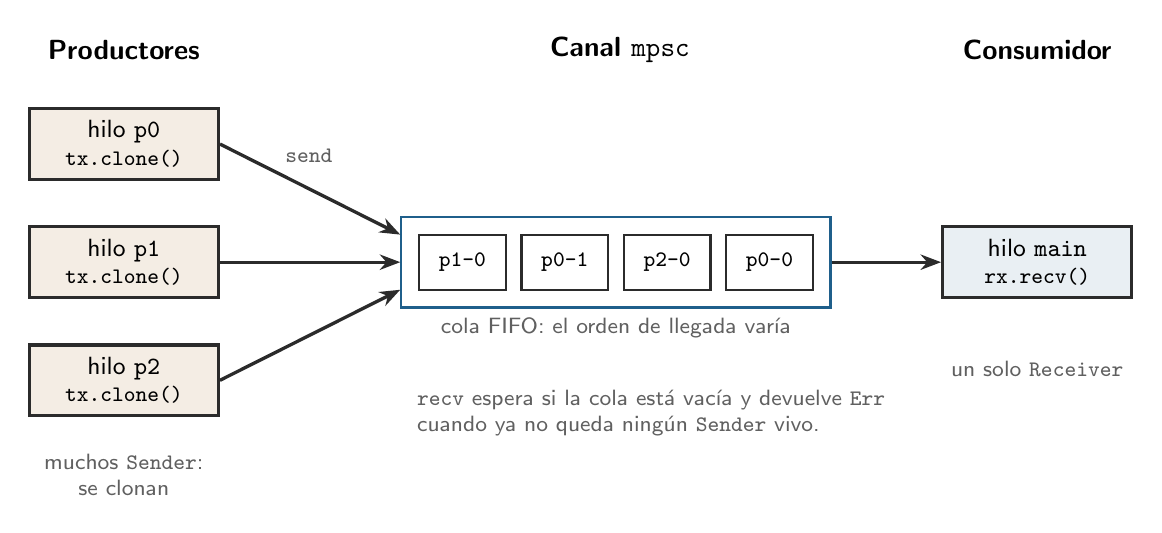
\begin{tikzpicture}[
  hilo/.style={draw=carbon,very thick,fill=arena,minimum width=24mm,minimum height=9mm,align=center,font=\sffamily\small},
  msj/.style={draw=carbon,thick,fill=white,minimum width=11mm,minimum height=7mm,font=\ttfamily\footnotesize},
  rotulo/.style={font=\sffamily\footnotesize\color{carbon!75}},
  >={Stealth[length=2.6mm]}]
  % Productores
  \node[font=\sffamily\bfseries] at (0,2.4) {Productores};
  \foreach \i/\y in {0/1.2,1/-0.3,2/-1.8} {
    \node[hilo] (p\i) at (0,\y) {hilo \texttt{p\i}\\[-1pt]{\footnotesize\ttfamily tx.clone()}};
  }
  % Cola del canal
  \node[font=\sffamily\bfseries] at (6.3,2.4) {Canal \texttt{mpsc}};
  \foreach \t [count=\k from 0] in {p1-0,p0-1,p2-0,p0-0} {
    \node[msj] (m\k) at (4.3+\k*1.3,-0.3) {\t};
  }
  \node[draw=azul,thick,inner sep=6pt,fit=(m0)(m3),label={[rotulo]below:cola FIFO: el orden de llegada varía}] (cola) {};
  % Consumidor
  \node[font=\sffamily\bfseries] at (11.6,2.4) {Consumidor};
  \node[hilo,fill=azul!10] (c) at (11.6,-0.3) {hilo \texttt{main}\\[-1pt]{\footnotesize\ttfamily rx.recv()}};
  % Flechas
  \foreach \i in {0,1,2} {
    \draw[->,very thick,carbon] (p\i.east) -- ($(cola.west)+(0,{0.35*(1-\i)})$);
  }
  \node[rotulo,fill=white,inner sep=1pt] at (2.35,1.05) {\texttt{send}};
  \draw[->,very thick,carbon] (cola.east) -- (c.west);
  % Notas
  \node[rotulo,align=center] at (0,-3.0) {muchos \texttt{Sender}:\\se clonan};
  \node[rotulo,align=center] at (11.6,-1.65) {un solo \texttt{Receiver}};
  \node[rotulo,align=left,anchor=north west] at (3.6,-1.8)
    {\texttt{recv} espera si la cola está vacía y devuelve \texttt{Err}\\cuando ya no queda ningún \texttt{Sender} vivo.};
\end{tikzpicture}
\end{document}
